% !TeX encoding = UTF-8
% !TeX root = choix_extensions.tex
\chapter{Maths}





\section{Extensions mathématiques particulièrement utiles}

Entre TeXstudio et le fichier \mintinline{latex}{preambule_college.sty}, il y a tout ce qu'il faut pour bien faire :
\begin{itemize}
	\item L'extension de \emph{l'American Mathematical Society} (AMS) \href{https://www.ctan.org/pkg/amsmath}{amsmath}, \href{https://www.ctan.org/tex-archive/fonts/amsfonts}{amsfonts}, \href{https://www.ctan.org/pkg/amsopn}{amsopn}.
	\item Les extensions suivantes sont très pratiques et méritent le coup d'{\oe}il :
		\begin{enumerate}
			\item  \href{https://www.ctan.org/tex-archive/macros/latex/contrib/IEEEtran/}{IEEEtran}
			\item \href{https://www.ctan.org/pkg/siunitx}{siunitx}
			\item \href{https://www.ctan.org/tex-archive/macros/latex/contrib/braket}{braket}
			\item \href{https://www.ctan.org/pkg/esvect}{esvect}.
		\end{enumerate}
	\item Avec TeXStudio, la plupart des symboles et des environnement mathématiques sont accessibles directement depuis les barres d'outils et le menu \mintinline{latex}{Math}.
\end{itemize}





\section{Paragraphes mathématiques spéciaux}

Pour mémoire (voir \ref{ch:paragraphesSpeciaux}), les paragraphes mathématiques les plus courants sont disponibles sous forme de raccourcis :
\begin{multicols}{3}
	\begin{itemize}
		\item \mintinline{latex}{\defin}
		\item \mintinline{latex}{\theoreme}
		\item \mintinline{latex}{\axiome}
		\item \mintinline{latex}{\hypothese}
		\item \mintinline{latex}{\these}
		\item \mintinline{latex}{\conclusion}
		\item \mintinline{latex}{\demonstration}
		\item \mintinline{latex}{\corollaire}
		\item \mintinline{latex}{\algorithme}
		\item \mintinline{latex}{\consequence}
	\end{itemize}
\end{multicols}

Ce qui donne en pratique :
\begin{multicols}{2}
	\defin[Titre]{A \emphdef{définir}}
	\theoreme[Titre]{Exemple}
	\axiome[Titre]{Exemple}
	\hypothese[Titre]{Exemple}
	\these[Titre]{Exemple}
	\conclusion[Titre]{Exemple}
	\demonstration[Titre]{Exemple}
	\corollaire[Titre]{Exemple}
	\algorithme[Titre]{Exemple}
\end{multicols}





\section{Alignements d'équations}
\label{sec:alignementEquations}

Pour les alignements plus précis, l'extension \href{http://mirror.ctan.org/macros/latex/contrib/IEEEtran/IEEEtran_HOWTO.pdf}{IEEEtran} fournit tous les outils nécessaires.

En particulier, on utilise l'environnement \mintinline{latex}{IEEEeqnarray} pour les alignements complexes. La syntaxe est similaire à celle d'un environnement \mintinline{latex}{tabular} ou \mintinline{latex}{array} (voir \ref{sec:tableauxMaths}).

Ainsi, on obtient : 
\[
	\begin{IEEEeqnarraybox}[][c]{rCrCl}
		\left.
		\begin{IEEEeqnarraybox}[\IEEEeqnarraystrutmode][c]{rCl?l}
			AB &=& CD & \text{(hyp)}\\
			OA &=& OD &(=r)\\
			OB &=& OC &(=r)
		\end{IEEEeqnarraybox}
		\, \right\}
		& \quad \xRightarrow{\parbox{.7cm}{\centering\scriptsize cas 3 iso}} \quad
		& BOA &\cong& DOC \\
		& \quad \xRightarrow{\parbox{1.5cm}{\centering\scriptsize thm angles au centre}} \quad
		& \wideparen{AB} &\cong& \wideparen{CD}
	\end{IEEEeqnarraybox}
\]

avec le code suivant :

\begin{minted}{latex}
\[
  \begin{IEEEeqnarraybox}[][c]{rCrCl}
    \left.
    \begin{IEEEeqnarraybox}[\IEEEeqnarraystrutmode][c]{rCl?l}
      AB &=& CD & \text{(hyp)}\\
      OA &=& OD &(=r)\\
      OB &=& OC &(=r)
    \end{IEEEeqnarraybox}
    \, \right\}
    & \quad \xRightarrow{\parbox{.7cm}{\centering\scriptsize cas 3 iso}} \quad
    & BOA &\cong& DOC \\
    & \quad \xRightarrow{\parbox{1.5cm}{\centering\scriptsize thm angles au
    centre}} \quad
    & \wideparen{AB} &\cong& \wideparen{CD}
  \end{IEEEeqnarraybox}
\]
\end{minted}

Dans cet environnement, on peut regrouper des colonnes avec \mintinline{latex}{\IEEEeqnarraymulticol}. Dans l'exemple suivant, on l'utilise pour aligner \mintinline{latex}{[AM] côté commun} :
\[
	\begin{IEEEeqnarraybox}[][c]{rCrCl?r}
		\left.
		\begin{IEEEeqnarraybox}[\IEEEeqnarraystrutmode][c]{rCl?l}
			\sphericalangle BAM &=& \sphericalangle MAC & ([AM) = b_{\alpha}) \\
			AB &=& AC & \text{(hyp)} \\
			\IEEEeqnarraymulticol{4}{c}{
				\left[AM\right] \text{côté commun}
			}
		\end{IEEEeqnarraybox}
		\, \right\}
		& \quad	\xRightarrow{\parbox{.7cm}{\centering\scriptsize cas 1 iso}} \quad &
		ABM &\cong& ACM \\
		& \quad \xRightarrow{\smash[t]{\text{déf}}} \quad &
		\sphericalangle CBA &=& \sphericalangle ACB &\qedhere
	\end{IEEEeqnarraybox}
\]

obtenu avec le code suivant :

\begin{minted}{latex}
\[
--- Le début du code a été omis ---
  \begin{IEEEeqnarraybox}[\IEEEeqnarraystrutmode][c]{rCl?l}
    \sphericalangle BAM &=& \sphericalangle MAC & ([AM) = b_{\alpha}) \\
    AB &=& AC & \text{(hyp)} \\
    \IEEEeqnarraymulticol{4}{c}{
      \left[AM\right] \text{côté commun}
    }
  \end{IEEEeqnarraybox}
--- La fin du code a été omise ---
\]
\end{minted}



Voir les détails dans le paragraphe sur \mintinline{latex}{IEEEeqnarray} dans \href{http://mirror.ctan.org/info/lshort/french/lshort-fr.pdf}{Une courte (?) introduction à \LaTeX$2\epsilon$} et dans la documentation de \href{http://mirror.ctan.org/macros/latex/contrib/IEEEtran/IEEEtran_HOWTO.pdf}{IEEEtran}.

Pour les cas simples, on peut utiliser \mintinline{latex}{array} (voir \ref{sec:tableauxMaths}). Dans tous les cas, il faut absolument éviter la commande \mintinline{latex}{eqnarray}).





\newpage





\section{Alignements d'exercices}
\label{sec:alignementExercices}

Pour composer des exercices sur plusieurs colonnes, on peut numéroter les exercices par colonne ou par ligne. Généralement, l'utilisation de l'espace est meilleure si on numérote par colonne.



\subsection{Numérotation en colonne (standard)}

Ce résultat est obtenu avec le code ci-dessous :
\exercice*{
	Résoudre :
	\begin{enumerate}[itemsep=1ex]
		\begin{multicols}{2}
			\item $\log_2(x) = 5$ 
			\item $2^{\ln(x)} = 3$ 
			\item $\log_3\left(\log_2(x)\right) = \num{0.5}$
			\item $\ln\left(x^2+3x+1\right) = -2$	
			\item $\log_3\left(x^2-x-1\right) = 1$
			\item $\log_x(5) = 2$
			\item $2\log(x-2)=\log(2x-4)$
			\item $\log_x\left(\dfrac{1}{3}\right)=2$
		\end{multicols}
	\end{enumerate}
}

\begin{minted}[gobble=1,tabsize=2]{latex}
	\exercice*{
		Résoudre :
		\begin{enumerate}[itemsep=1ex]
			\begin{multicols}{2}
				\item $\log_2(x) = 5$ 
				\item $2^{\ln(x)} = 3$ 
				\item $\log_3\left(\log_2(x)\right) = \num{0.5}$
				\item $\ln\left(x^2+3x+1\right) = -2$		
				\item $\log_3\left(x^2-x-1\right) = 1$
				\item $\log_x(5) = 2$
				\item $2\log(x-2)=\log(2x-4)$
				\item $\log_x\left(\dfrac{1}{3}\right)=2$
			\end{multicols}
		\end{enumerate}
	}
\end{minted}

\remarque*{
	De cette manière l'espace est utilisé au mieux, mais les expressions dans les deux colonnes ne sont pas forcément alignées : ce n'est pas un tableau\dots
}



\subsection{Numérotation en colonne sur peu de lignes}

S'il y a peu de lignes et que certaines expressions sont verticalement bien plus grandes que d'autres, des décalages verticaux gênants peuvent apparaître avec \inlatex{multicols}. Dans ce cas, on force l'alignement horizontal en ne tenant pas compte de la hauteur des expressions mathématiques (avec \inlatex{\smash}) et en gérant les espaces interlignes avec \inlatex{itemsep} en option de l'environnement \inlatex{enumerate} :

Par exemple :

\exercice*{
	Soit l'ensemble $E$ des six fonctions suivantes de $\R \smallsetminus \set{0;1}$ vers $\R\smallsetminus \set{0;1}$ :
	\begin{enumerate}[itemsep=2ex]
		\begin{multicols}{3}
			\item[] $\smash{f_1 : x \mapsto x}$
			\item[] $\smash{f_2 : x \mapsto \dfrac{1}{x}}$
			\item[] $\smash{f_3 : x \mapsto 1-x}$
			\item[] $\smash{f_4 : x \mapsto \dfrac{1}{1-x}}$
			\item[] $\smash{f_5 : x \mapsto \dfrac{x-1}{x}}$
			\item[] $\smash{f_6 : x \mapsto \dfrac{x}{x-1}}$
		\end{multicols}
	\end{enumerate}
	Montrer que $(E,\circ)$ est un groupe. Est-il abélien ?
}

Produit par le code :

\begin{minted}[gobble=1,tabsize=2]{latex}
	\exercice{
		Soit l'ensemble $E$ des six fonctions suivantes de $\R \smallsetminus \set{0;1}$ vers $\R\smallsetminus \set{0;1}$ :
		\begin{enumerate}[itemsep=2ex]
			\begin{multicols}{3}
				\item[] $\smash{f_1 : x \mapsto x}$
				\item[] $\smash{f_2 : x \mapsto \dfrac{1}{x}}$
				\item[] $\smash{f_3 : x \mapsto 1-x}$
				\item[] $\smash{f_4 : x \mapsto \dfrac{1}{1-x}}$
				\item[] $\smash{f_5 : x \mapsto \dfrac{x-1}{x}}$
				\item[] $\smash{f_6 : x \mapsto \dfrac{x}{x-1}}$
			\end{multicols}
		\end{enumerate}
		Montrer que $(E,\circ)$ est un groupe. Est-il abélien ?
	}
\end{minted}



\subsection{Numérotation en une ligne}

Pour les alignement en une seule ligne, on peut se passer de \inlatex{multicols} et utiliser directement les environnements étoilés de l'extension \inlatex{enumitem} :

Par exemple :

\exercice*{
	Résoudre : \\[1ex]
	\begin{enumerate*}[itemjoin=\hfill,label=\arabic*),afterlabel=\quad]
		\item $\log_3\left(x^2-x-1\right) = 1$
		\item $\log_x(5) = 2$
		\item $2\log(x-2)=\log(2x-4)$
		\item $\log_x\left(\dfrac{1}{3}\right)=2$
	\end{enumerate*}
}

Produit par le code

\begin{minted}[gobble=1,tabsize=2]{latex}
\exercice*{
	Résoudre : \\[1ex]
	\begin{enumerate*}[itemjoin=\hfill,label=\arabic*),afterlabel=\quad]
		\item $\log_3\left(x^2-x-1\right) = 1$
		\item $\log_x(5) = 2$
		\item $2\log(x-2)=\log(2x-4)$
		\item $\log_x\left(\dfrac{1}{3}\right)=2$
	\end{enumerate*}
}
\end{minted}

\remarque*{
	Pour générer des listes d'exercices dont la numérotation est en ligne, on peut utiliser l'extension \href{https://www.ctan.org/pkg/tasks}{tasks}.
}





\section{Nombres avec unités}

Pour les unités, l'extension \href{http://mirror.ctan.org/macros/latex/contrib/siunitx/siunitx.pdf}{siunitx} offre des fonctionnalités très pratiques :
\begin{LTXexample}[pos=o,width=.4]
Unités indifféremment en mode text, \SI{25}{kJ} ou maths, $E = \SI{25}{kJ}$ \\
Notation scientifique : \SI{4.35e-12}{kg} \\
Unité seule : \si{\degree} \\
Nombre seul : \num{25,3}
\end{LTXexample}

Dans le dernier exemple, notez que le code contient une virgule décimale, alors que le texte compilé contient un point décimal. C'est un exemple des nombreux paramètres que l'on peut régler avec \href{http://mirror.ctan.org/macros/latex/contrib/siunitx/siunitx.pdf}{siunitx}.

Ici, le fichier \mintinline{latex}{preambule_college.sty} contient :
\begin{minted}{latex}
\sisetup{
  output-decimal-marker={.},
}
\end{minted}





\section{Réponses optionnelles aux exercices}

Dans les exercices, on peut lier une réponse à chaque question et la faire afficher avec l'option de compilation \mintinline{latex}{reponse}. Pour cela, le préambule du document doit contenir \mintinline{latex}{\usepackage[reponse]{optional}}. Ceci permet d'activer les raccourcis suivants de  \incmd{preambule_college.sty} :

\begin{enumerate}
	\item \mintinline{latex}{\rep{expression}} : une réponse (expression mathématique requise en argument);
	\item \mintinline{latex}{\rept{text}} : une réponse sous forme de texte (mais pas de liste);
	\item \mintinline{latex}{\repl{liste}} : une réponse texte, y.c. sous forme de liste (basé sur minipage);
	\item \mintinline{latex}{\repn{valeur}} : une réponse numérique, en particulier à virgule basée sur \mintinline{latex}{\num} de l'extension \incmd{siunitx};
	\item \mintinline{latex}{\repSI{valeur}{unité}} : une réponse basée sur \mintinline{latex}{\SI} de l'extension \incmd{siunitx};
	\item \mintinline{latex}{\repNewline} : un \mintinline{latex}{\newline} seulement actif avec les réponses.
\end{enumerate}

\begin{minipage}{.63\linewidth}
	\begin{minted}{latex}
\documentclass{report}
\usepackage{preambule_college}
\usepackage[reponse]{optional}
\begin{document}
\begin{enumerate}
  \begin{multicols}{2}
    \item $\sqrt{6400} =$ $\rep{80}$
    \item Une année-lumière. \repSI{9,45e12}{km}
    \item $(2x+1)(4x-5)=0$\repNewline
      $\rep{S=\Set{-\dfrac{1}{2}; \dfrac{5}{4}}}$
    \item $\num{0,005} \cdot \num{0,06}
      = \repn{3e-4}$
    \item $(x+2)(x-3)(2x-5)(x-\sqrt{3})=0$\repNewline
      \repl{$S_{\N}=\Set{3}$\\ $S_{\Z}=\Set{-2; 3}$\\
        $S_{\Q}=\Set{-2; 3; \cfrac{5}{2}}$\\
        $S_{\R}=\Set{-2; 3; \cfrac{5}{2}; \sqrt{3}}$
      }
  \end{multicols}
\end{enumerate}
\end{document}
	\end{minted}
\end{minipage}
\hfill
\begin{minipage}{.35\linewidth}
	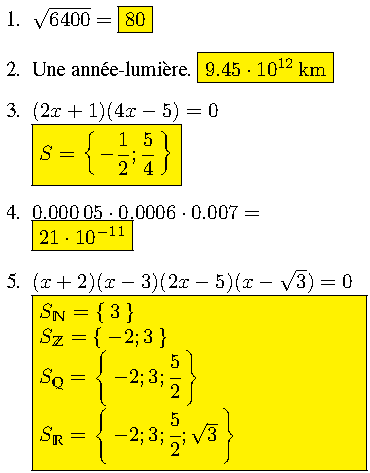
\includegraphics{images/choix_extensions_exemple_reponses}
\end{minipage}




\section{Symboles}



\subsection{Trouver efficacement des symboles}

Pour trouver des symboles, on peut :
\begin{enumerate}
	\item Utiliser les barres d'outils de TeXstudio.
	\item Parcourir \href{https://www.ctan.org/tex-archive/info/symbols/comprehensive/}{The Comprehensive \LaTeX Symbol List}. Pour cela, il faut soit connaître le nom anglais du symbole, soit être patient\dots
	\item Le site \href{http://webdemo.myscript.com}{\url{http://webdemo.myscript.com}} propose l'outil "Web Equation" qui permet d'écrire à la main une formule et vous donne la traduction \LaTeX.
	\item Dessiner son symbole dans \href{http://detexify.kirelabs.org/classify.html}{detexify}. Detexify est aussi disponible pour iOS et pour Android, ce qui permet de dessiner à la main et non à la souris !
\end{enumerate}



\subsection{Symboles mathématiques en gras}

Pour mettre un symbole en gras, par exemple dans un titre, on utilise \inlatex{\symbf} avec l'extension \incmd{unicode-math}. 
\begin{LTXexample}[pos=o,width=.3]
\subsubsection*{Le nombre $\pi$}
\subsubsection*{Le nombre ${\symbf\pi}$}
\end{LTXexample}

Anciennement, on utilisait soit \inlatex{\mathbf{}}, soit \inlatex{\bm} de l'extension du même nom.


Pour mettre un symbole en gras dans un titre de chapitre, dans l'en-tête, mais pas dans la table des matières : \mintinline{latex}{{\boldmath\SI[detect-weight]{0}{\degree}}}



\vspace*{\topsep}
\subsection{Symboles faits maison}

Le fichier \mintinline{latex}{preambule_college.sty} comporte des raccourcis permettant de faire des symboles divers non définis en standard :
\begin{LTXexample}[pos=o,width=.3]
\nRe                \\% pas en relation avec
\nsubset            \\% non inclus
\nbot               \\% non perpendiculaire
\nLeftrightarrow	\\% non équivalent
\vide               \\% ensemble vide un peu plus joli...
\ie                 \\% id est 
\de                 \\% °, basé sur siunitx
\Hyp                \\% pour introduire une hypothèse
\The                \\% pour introduire une thèse
\Dem                \\% pour introduire une démonstration
\nondef				  % pour les valeurs "non définies" dans les tables de signe
\end{LTXexample}



\subsection{Divers symboles}


\subsubsection{Symboles pour les arcs}

En utilisant directement les accents de la police mathématique\footnote{Il faut donc que la police les ait\dots \ Pour l'instant, seules celles accessibles par les commandes \inlatex{\mathversion} de \incmd{preambule_personnalisation.sty} fonctionnent correctement.}.

\begin{LTXexample}[pos=o,width=.3]
$\wideparen{ABC}$
\end{LTXexample}


En utilisant l'extension \href{https://www.ctan.org/pkg/mathtools}{mathtools} :
\begin{LTXexample}[pos=o,width=.3]
$\xRightarrow{\parbox{.7cm}{\centering\scriptsize cas 3}}$
\end{LTXexample}


\subsubsection{Symboles récupérés}

Certains symboles sont liés à une police de caractère, notamment \mintinline{latex}{Palatino}. Le fichier \mintinline{latex}{prambule_college.sty} en récupère quelques-uns sans qu'il n'y ait besoin de changer toute la police de caractères :

\begin{LTXexample}[pos=o,width=.3]
$\varparallel$  \\ % parallèle (penché à droite)
$\nvarparallel$    %non parallèle (penché à droite)
\end{LTXexample}





\section{Raccourcis divers}



\subsection{Fractions}

Pour varier le style des fractions, on utilise les extensions AMS et \href{http://mirror.ctan.org/macros/latex/contrib/l3packages/xfrac.pdf}{xfrac}.
\begin{LTXexample}[pos=o,width=.3]
$\dfrac{1}{2}$ \\[1ex]
$\sfrac{1}{2}$ \\[1ex]
$\cfrac{1}{2}$
\end{LTXexample}

\mintinline{latex}{\cfrac} se comporte bien dans les fractions de fraction. Par ailleurs, pour les cas désespérés dans lesquels l'espacement autour de la barre de fraction doit être réglé finement :
\begin{LTXexample}[pos=o,width=.15]
$\genfrac{}{}{0.9pt}{0}{3\cdot \dfrac52 + \dfrac39} {2-\dfrac{-8}{12}}$
\end{LTXexample}




\subsection{Barrer des expressions}

Pour barre une expression mathématique, on peut utiliser l'extension \href{http://mirror.ctan.org/macros/latex/contrib/cancel/cancel.pdf}{cancel}.

\begin{LTXexample}[pos=o,width=.3]
$\dfrac{2x^{\cancel{2}}}{\cancel{x}}$
\end{LTXexample}



\subsection{Valeur absolue, norme}

Ces raccourcis définis selon \href{http://mirror.ctan.org/macros/latex/contrib/mh/mathtools.pdf}{mathtools} permettent de gérer l'espacement horizontal et la hauteur des barres, automatiquement ou à la main (avec \inlatex{\big}, \inlatex{\Big}, \inlatex{\bigg} ou \inlatex{\Bigg}) :

\begin{LTXexample}[pos=o,width=.3]
$\abs*{\frac{3}{4}}$ \\[1ex]
$\norm*{\frac{x^2}{y^2}}$ \\[1ex]
$\abs[\Big]{\frac{3}{4}}$ \\[1ex]
$\norm[\bigg]{\frac{x^2}{y^2}}$
\end{LTXexample}



\subsection{Réciproque}

\begin{LTXexample}[pos=o,width=.3]
$\recip{G}$
\end{LTXexample}



\subsection{Barre sur une expression}

Pour avoir un peu plus d'espace entre la barre et l'expression :
\begin{LTXexample}[pos=o,width=.3]
$\ovline{P \text{ ou } Q}$
\end{LTXexample}

Pour la composition des nombres périodiques :
\begin{LTXexample}
	$\SI[parse-numbers=false]{0,\overline{1234}}{m^2}$
\end{LTXexample}




\subsection{Ensembles et intervalles}
Les ensembles sont faits avec \mintinline{latex}{\set} (hauteur fixe) et \mintinline{latex}{\Set} (hauteur variable) de l'extension \incmd{braket} :

\begin{LTXexample}[pos=o,width=.3]
$\set{x \in \N | x^2-1=0}$ \\[1ex]
$\Set{x \in \N | \dfrac{x}{2} \in \N}$
\end{LTXexample}

Pour les intervalles : toujours utiliser \mintinline{latex}{\left} et \mintinline{latex}{\right} avec les crochets, sinon il y a un problème d'espacement avant et après les \mintinline{latex}{[]}. Ca permet aussi de les retrouver plus facilement dans le code.

\remarque*{
	Barre verticale hors des ensembles : \mintinline{latex}{\mid} est la même chose que \mintinline{latex}{\;|\;}, et dans un \mintinline{latex}{\left... \right...} on peut utiliser \mintinline{latex}{\middle} à la place de \mintinline{latex}{\mid} pour avoir une hauteur variable. Sinon, \mintinline{latex}{\;\big|\;}.
}



\subsection{Systèmes d'équations}

Réalisés avec l'extension \incmd{IEEEtrantools} pour pouvoir gérer finement les alignements :

\begin{LTXexample}[pos=o,width=.3]
$\left\{ \,
\begin{IEEEeqnarraybox}[][c]{cCc}
  \IEEEstrut
  \frac{x}{2} - \frac{1}{3} &>& \frac{2-x}{4} \\[1ex]
  3x(x-2) &\leqslant& x^2 - 2x
  \IEEEstrut
\end{IEEEeqnarraybox}
\right.$
\end{LTXexample}

\begin{LTXexample}[pos=o,width=.3]
$\left\{ \,
\begin{IEEEeqnarraybox}[][c]{cCcCc?c}
  \IEEEstrut
  7x &-& 2y &=& 4 & (1)\\
  -4x &+& 5y &=& 17 & (2)
  \IEEEstrut
\end{IEEEeqnarraybox}
\right.$
\end{LTXexample}

Pour mémoire : un extrait de la documentation de \incmd{IEEEeqnarraybox} :


\subsubsection{Descripteurs de colonnes}

\setlength\extrarowheight{3pt}
\begin{tabular}{|c|l||c|l|}
	\hline
	I.D. & Description & I.D. & Description \tabularnewline
	\hline
	l & left math & v & vertical rule \tabularnewline
	c & centered math & vv & two vertical rule \tabularnewline
	r & right math & V & double vertical rule \tabularnewline
	L & left math with ords & VV & two double vertical rule \tabularnewline
	C & centered math with ords & h & horizontal rule\tabularnewline
	R & right math with ords & H & double horizontal rule\tabularnewline
	s & left text & x & empty \tabularnewline
	t & centered text & X & empty math \tabularnewline
	u & right text & & \tabularnewline
	\hline
\end{tabular}


\subsubsection{Descripteurs des séparations}

\begin{tabular}{|c|l||c|l|}
	\hline
	I.D. & Description & I.D. & Description \tabularnewline
	\hline
	! & $-\sfrac{1}{6}$ em & . & \mintinline{latex}{0.5\arraycolsep} \tabularnewline
	, & $\sfrac{1}{6}$ em  & / & \mintinline{latex}{1.0\arraycolsep} \tabularnewline
	: & $\sfrac{2}{9}$ em  & ? & \mintinline{latex}{2.0\arraycolsep} \tabularnewline
	; & $\sfrac{5}{18}$ em  & * & 9pt plus 1fil\tabularnewline
	' & 1 em & + & 1000pt minus 1000pt\tabularnewline
	" & 1 em & - & 0 pt\tabularnewline
	\hline
\end{tabular}


\subsubsection{Espacement des lignes les tableaux}
Pour gérer l'espacement des lignes dans un \mintinline{latex}{IEEEeqnarray} :
\begin{enumerate}
	\item \mintinline{latex}{\IEEEvisiblestrutstrue} pour voir les struts invisibles;
	\item \mintinline{latex}{\IEEEeqnarraystrutsize} and \mintinline{latex}{\IEEEeqnarraystrutsizeadd} pour gérer la hauteur, à placer dans \newline \mintinline{latex}{\begin{IEEEeqnarraybox}[\IEEEeqnarraystrutsize{2ex}{0ex}]}
\end{enumerate}



\subsection{Limites}

\begin{LTXexample}[pos=o,width=.3]
\Lim{1}{2}    %lim
\Limd{1}{2}   %lim plus (ou à droite)
\Limg{1}{2}   %lim moins (ou à gauche)
\end{LTXexample}



\subsection{Vecteurs}

Pour les flèches sur les vecteurs, on utilise l'extension \href{http://mirror.ctan.org/macros/latex/contrib/esvect/esvect.pdf}{esvect}. En appelant l'extension avec une option, on peut choisir la forme de la flèche, ici le \mintinline{latex}{d} : \mintinline{latex}{\usepackage[d]{esvect}} (voir la documentation de \href{http://mirror.ctan.org/macros/latex/contrib/esvect/esvect.pdf}{esvect} pour plus de détail).

Les commandes de base sont : 
\begin{LTXexample}[pos=o,width=.3]
Vecteur quelconque  : $\vv{m}$ ou $\ve{m}$\\
Vecteur avec indice : $\vv*{e}{1}$
\end{LTXexample}

Raccourcis pour les vecteurs courants (avec ou sans les \$) :
\begin{LTXexample}[pos=o,width=.3]
$\va$   $\vb$ $\vc$  $\vd$  $\vn$ $\vu$ \\
$\vvv$ $\vo$ $\veu$ $\ved$ $\vet$
\end{LTXexample}

Raccourcis pour les vecteurs à deux (d) ou trois (t) composantes, avec des crochets :
\begin{LTXexample}[pos=o,width=.3]
$\compd{1}{2}$       %2 composantes
$\compt{1}{2}{3}$   %3 composantes
$\comb{1}{2}{3}$     %3 composantes avec [] brackets
\end{LTXexample}



\subsection{Matrices et déterminants}

\begin{LTXexample}[pos=o,width=.4]
$\matd{1}{2}{3}{4}$
$\matt{1}{2}{3}{4}{5}{6}{7}{8}{9}$
$\detd{1}{2}{3}{4}$
$\dett{1}{2}{3}{4}{5}{6}{7}{8}{9}$
\end{LTXexample}

Si on doit colorer de matrices, il vaut mieux utiliser les modules de TikZ.

\begin{LTXexample}[pos=o,width=.4]
\[
\begin{tikzpicture}
  \matrix (C){
    1 & -2 & 1  \\
    0 & 2  & -8 \\
    5 & 0  & -5 \\
 };
 \node[right=0 of C] (F) {$\cdot$};
 \matrix[right=0.1em of F] (X){
    x_1 \\
    x_2 \\
    x_3 \\
 };
 \node[right=0 of X] (E) {$=$};
 \matrix[right=0.1em of E] (P){
    x_1-2 x_2+x_3 \\
    2 x_2-8 x_3 \\
    5 x_1-5 x_3 \\
 };
  \begin{scope}[on background layer]
   \filldraw[cyan!50, rounded corners] (C-1-1.north west) -- (C-1-1.south west) -- (C-1-3.south east) --(C-1-3.north east)-- cycle;
   \filldraw[cyan!50, rounded corners] (X-1-1.north west) -- (X-3-1.south west) -- (X-3-1.south east) -- (X-1-1.north east) -- cycle;
   \filldraw[cyan!50, rounded corners] (P-1-1.north west) -- (P-1-1.south west) -- (P-1-1.south east)-- (P-1-1.north east)-- cycle;
  \end{scope}
\end{tikzpicture}
\]
\end{LTXexample}



\subsection{Tableaux des signes et des variations}

Avec l'extension \incmd{tkz-tab.sty}. L'exemple suivant est généré avec ce code :

\begin{minted}{latex}
\begin{tikzpicture}
  \tkzTabInit[lgt=4,espcl=3.5]{$x$/1.2,$a$/1.2,$x-x_1$/1.2,$x-x_2$/1.2,
    $a \left(x - x_1\right) \left(x -x_2\right)$/1.2}{$-\infty$,$x_1$,$x_2$,$+\infty$}
  \tkzTabLine{,$\text{signe de} a$,,$\text{signe de} a$,,$\text{signe de} a$,}
  \tkzTabLine{,-,0,+,,+,}
  \tkzTabLine{,-,,-,0,+,}
  \tkzTabLine{,$\text{signe de} a$,0,$-~\text{signe de} a$,0,$\text{signe de} a$,}
\end{tikzpicture}
\end{minted}

\begin{tikzpicture}
	\tkzTabInit[lgt=4,espcl=3.5]{$x$/1.2,$a$/1.2,$x-x_1$/1.2,$x-x_2$/1.2,$a \left(x - x_1\right) \left(x -x_2\right)$/1.2}{$-\infty$,$x_1$,$x_2$,$+\infty$}
	\tkzTabLine{,$\text{signe de} a$,,$\text{signe de} a$,,$\text{signe de} a$,}
	\tkzTabLine{,-,0,+,,+,}
	\tkzTabLine{,-,,-,0,+,}
	\tkzTabLine{,$\text{signe de} a$,0,$-~\text{signe de} a$,0,$\text{signe de} a$,}
\end{tikzpicture}


\begin{minted}{latex}
\begin{tikzpicture}
	\tkzTabInit[nocadre,lgt = 1.5, espcl = 2.5, deltacl=.1]
	{$x$ /0.8, $f'(x)$ /0.8, $f''(x)$ /0.8, $f(x)$ /0.8, $~$ /0.8}
	{ ,$a$,$b$,$c$, }
	\tkzTabLine{  ,+, z ,- , , -,  z,+, }
	\tkzTabLine{  ,-,  ,- , z , +,  ,+, }
	\tkzTabVar{  -/, +/ M / ,  R/  /,   -/ m /,+/, }
	\tkzTabLine{  ,\frown ,  , \frown , I , \smile , , \smile }
\end{tikzpicture}
\end{minted}

\begin{tikzpicture}
	\tkzTabInit[nocadre,lgt = 1.5, espcl = 2.5, deltacl=.1]
	{$x$ /0.8, $f'(x)$ /0.8, $f''(x)$ /0.8, $f(x)$ /0.8, $~$ /0.8}
	{ ,$a$,$b$,$c$, }
	\tkzTabLine{  ,+, z ,- , , -,  z,+, }
	\tkzTabLine{  ,-,  ,- , z , +,  ,+, }
	\tkzTabVar{  -/, +/ M / ,  R/  /,   -/ m /,+/, }
	\tkzTabLine{  ,\frown ,  , \frown , I , \smile , , \smile }
\end{tikzpicture}



\subsection{Ensembles, groupes\dots}

\begin{LTXexample}[pos=o,width=.3]
$\R$ $\Q$ $\CC$ $\N$ $\Z$ $\A$ $\BB$ $\P$ $\I$ $\D$
\end{LTXexample}

Malheureusement, les commandes \mintinline{latex}{\C} et \mintinline{latex}{\B} sont déjà définies.



\subsection{Notations calligraphiques}

\begin{LTXexample}[pos=o,width=.3]
$\cA$ $\cB$ $\cC$ $\cD$ $\cE$ $\cF$ $\cG$ $\cH$ $\cI$
$\cJ$ $\cK$ $\cL$ $\cM$ $\cN$ $\cO$ $\cP$ $\cQ$ $\cR$
$\cS$ $\cT$ $\cU$ $\cV$ $\cW$ $\cX$ $\cY$ $\cZ$
\end{LTXexample}



\subsection{Typographies spéciales en mode mathématique}

\begin{LTXexample}[pos=o,width=.25]
$\ppmc$ $\pgdc$ $\sgn$ $\Alt$ $\fix$ $\card$ $\rang$ $\dom$
$\vect$ $\diag$ $\supp$ $\ind$ $\im{f}$ $\codim$ $\sign$ $\tr$
$\id$ $\GL$ $\SL$ $\car$ $\perm$
\end{LTXexample}






\section{Quelques curiosités}

Parfois, il est utile d'écrire une expression qui ne compte pas dans le calcul des largeurs et des centrages; cette boîte est de largeur nulle dans la composition des textes voisins.
\begin{enumerate}
	\item \mintinline{latex}{\mathllap{expr}} : la boîte part sur la gauche;
	\item \mintinline{latex}{\mathclap{expr}} : la boîte est centrée;
	\item \mintinline{latex}{\mathrlap{expr}} : la boîte part sur la droite
\end{enumerate}
\begin{LTXexample}[pos=o,width=.3]
\begin{center}
$\mathllap{\pi+\sqrt{5}}$ texte centré\\
texte $\mathclap{\pi+\sqrt{5}}$ centré\\
texte centré $\mathrlap{\pi+\sqrt{5}}$
\end{center}
\end{LTXexample}

Ces commandes peuvent compléter celles-ci : \mintinline{latex}{\smash}, \mintinline{latex}{\phantom}, \mintinline{latex}{code}, \mintinline{latex}{\vphantom}, \mintinline{latex}{\hphantom}, \mintinline{latex}{\llap}, \mintinline{latex}{\clap} et \mintinline{latex}{\rlap}.

